
\chapquote{``In order to understand recursion, one must first understand recursion."}{Anonymous}

\problem The \textit{Tower of Hanoi} is a mathematical puzzle, consisting of three rods and a number of disks of different sizes which
can slide onto any rod. The puzzle starts with all disks, in ascending order of size, on one rod. The objective of the puzzle is to
move the entire stack to another rod, obeying the foolowing rules.
\begin{enumerate}
	\item Only one disk can be moved at a time.
	\item Each move consists of taking the upper disk from one stack and placing it on the top of another stack or empty rod.
	\item No disk can be placed on a smaller disk.
\end{enumerate}
\begin{figure}[h]
	\begin{center}
		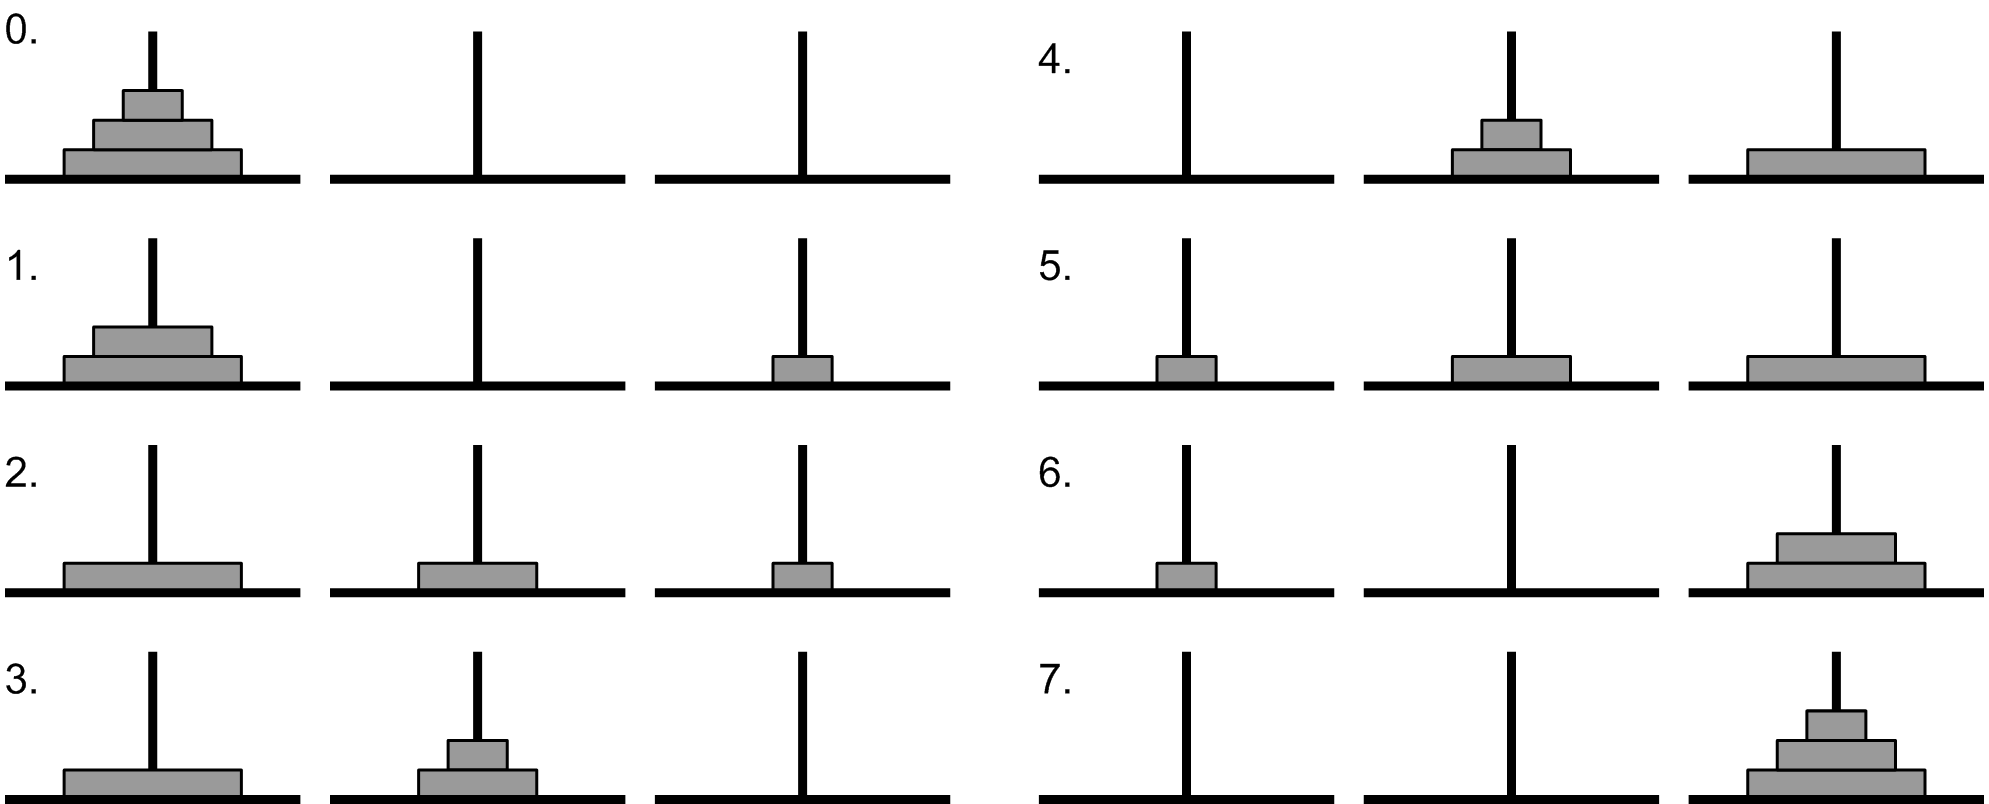
\includegraphics[scale=0.7]{hanoi.png}
	\end{center}
	\caption*{Solution to the Towers of Hanoi with 3 disks.}
	\label{fig:hanoi_solved}
\end{figure}

Solve the \textit{Tower of Hanoi} puzzle for an arbitrary number of disks, enumerating the required moves.

\solution The main insight here is that the problem involving $n$ disks can be reduced to one with $n - 1$ disks.
Labelling the rods $A$, $B$ and $C$, and the disks with numerals $1$ through $n$ (smallest to largest), our aim is to move the
entire stack from $A$ to $C$. If we can solve the problem with $n - 1$ disks, all we have to do is to move the topmost $n - 1$ disks
from $A$ to $B$, move the remaining disk on $A$ to $C$, and again move the $n - 1$ disks on $B$ to $C$. The base case for this
recursive solution is moving $1$ disk, which is trivial.

Clearly, if the problem with $n$ disks takes $k_n$ number of moves, the problem with $n + 1$ moves will take $k_n + 1 + k_n = 2k_n + 1$ moves.
For the base case with one disk, $k_1 = 1$. With this infromation, we see that the \textit{Tower of Hanoi} with $n$ disks can be solved
in exactly $2^n - 1$ moves.

\algorithm
\texttt{main (disks:Integer)}
\begin{enumerate}
	\item Call \texttt{solveHanoi(disks, "A", "C", "B")}.
	\item \textbf{Exit} 
\end{enumerate}
\vspace{5mm}
\texttt{solveHanoi (disk:Integer, source:String, destination:String, spare:String)}
\begin{enumerate}
	\item If \texttt{disk} is zero, \textbf{return}.
	\item Call \texttt{solveHanoi(disk - 1, source, spare, destination)}.
	\item Move disk number \texttt{disk} has to be moved from \texttt{source} to \texttt{destination}.
	\item Call \texttt{solveHanoi(disk - 1, spare, destination, source)}.
	\item \textbf{Return} 
\end{enumerate}

\sourcecode
\lstinputlisting{src/TowersOfHanoi.java}

\varDescription
\begin{longtable} {| >{\ttfamily}p{0.16\linewidth} | >{\ttfamily}p{0.2\linewidth}| p{0.6\linewidth} |}
\hline\multicolumn{3}{|c|}{\tt TowersOfHanoi::main(String[])} 		\\\hline
int 		&	disks	&	The number of disks in the problem \\\hline
\hline\multicolumn{3}{|c|}{\tt TowersOfHanoi::solveHanoi(int, String, String, String)} 		\\\hline
int 		&	disk	&	The current disk to be moved \\\hline
String		&	source	&	The rod from which the stack is to be moved\\\hline
String		&	destination&	The rod to which the stack is to be moved \\\hline
String		&	spare	&	The additional rod, where the remaining \texttt{n-1} disks are temporarily moved  \\\hline 
\end{longtable}
